\documentclass{beamer}

% xcolor and define colors -------------------------
\usepackage{xcolor}

% https://www.viget.com/articles/color-contrast/
\definecolor{purple}{HTML}{5601A4}
\definecolor{navy}{HTML}{0D3D56}
\definecolor{ruby}{HTML}{9a2515}
\definecolor{alice}{HTML}{107895}
\definecolor{daisy}{HTML}{EBC944}
\definecolor{coral}{HTML}{F26D21}
\definecolor{kelly}{HTML}{829356}
\definecolor{cranberry}{HTML}{E64173}
\definecolor{jet}{HTML}{131516}
\definecolor{asher}{HTML}{555F61}
\definecolor{slate}{HTML}{314F4F}

% Mixtape Sessions
\definecolor{picton-blue}{HTML}{00b7ff}
\definecolor{violet-red}{HTML}{ff3881}
\definecolor{sun}{HTML}{ffaf18}
\definecolor{electric-violet}{HTML}{871EFF}

% Main theme colors
\definecolor{accent}{HTML}{00b7ff}
\definecolor{accent2}{HTML}{871EFF}
\definecolor{gray100}{HTML}{f3f4f6}
\definecolor{gray800}{HTML}{1F292D}


% Beamer Options -------------------------------------

% Background
\setbeamercolor{background canvas}{bg = white}

% Change text margins
\setbeamersize{text margin left = 15pt, text margin right = 15pt} 

% \alert
\setbeamercolor{alerted text}{fg = accent2}

% Frame title
\setbeamercolor{frametitle}{bg = white, fg = jet}
\setbeamercolor{framesubtitle}{bg = white, fg = accent}
\setbeamerfont{framesubtitle}{size = \small, shape = \itshape}

% Block
\setbeamercolor{block title}{fg = white, bg = accent2}
\setbeamercolor{block body}{fg = gray800, bg = gray100}

% Title page
\setbeamercolor{title}{fg = gray800}
\setbeamercolor{subtitle}{fg = accent}

%% Custom \maketitle and \titlepage
\setbeamertemplate{title page}
{
    %\begin{centering}
        \vspace{20mm}
        {\Large \usebeamerfont{title}\usebeamercolor[fg]{title}\inserttitle}\\
        {\large \itshape \usebeamerfont{subtitle}\usebeamercolor[fg]{subtitle}\insertsubtitle}\\ \vspace{10mm}
        {\insertauthor}\\
        {\color{asher}\small{\insertdate}}\\
    %\end{centering}
}

% Table of Contents
\setbeamercolor{section in toc}{fg = accent!70!jet}
\setbeamercolor{subsection in toc}{fg = jet}

% Button 
\setbeamercolor{button}{bg = accent}

% Remove navigation symbols
\setbeamertemplate{navigation symbols}{}

% Table and Figure captions
\setbeamercolor{caption}{fg=jet!70!white}
\setbeamercolor{caption name}{fg=jet}
\setbeamerfont{caption name}{shape = \itshape}

% Bullet points

%% Fix left-margins
\settowidth{\leftmargini}{\usebeamertemplate{itemize item}}
\addtolength{\leftmargini}{\labelsep}

%% enumerate item color
\setbeamercolor{enumerate item}{fg = accent}
\setbeamerfont{enumerate item}{size = \small}
\setbeamertemplate{enumerate item}{\insertenumlabel.}

%% itemize
\setbeamercolor{itemize item}{fg = accent!70!white}
\setbeamerfont{itemize item}{size = \small}
\setbeamertemplate{itemize item}[circle]

%% right arrow for subitems
\setbeamercolor{itemize subitem}{fg = accent!60!white}
\setbeamerfont{itemize subitem}{size = \small}
\setbeamertemplate{itemize subitem}{$\rightarrow$}

\setbeamertemplate{itemize subsubitem}[square]
\setbeamercolor{itemize subsubitem}{fg = jet}
\setbeamerfont{itemize subsubitem}{size = \small}







% Links ----------------------------------------------

\usepackage{hyperref}
\hypersetup{
  colorlinks = true,
  linkcolor = accent2,
  filecolor = accent2,
  urlcolor = accent2,
  citecolor = accent2,
}


% Line spacing --------------------------------------
\usepackage{setspace}
\setstretch{1.2}


% \begin{columns} -----------------------------------
\usepackage{multicol}


% Fonts ---------------------------------------------
% Beamer Option to use custom fonts
\usefonttheme{professionalfonts}

% \usepackage[utopia, smallerops, varg]{newtxmath}
% \usepackage{utopia}
\usepackage[sfdefault,light]{roboto}

% Small adjustments to text kerning
\usepackage{microtype}



% Remove annoying over-full box warnings -----------
\vfuzz2pt 
\hfuzz2pt


% Table of Contents with Sections
\setbeamerfont{myTOC}{series=\bfseries, size=\Large}
\AtBeginSection[]{
        \frame{
            \frametitle{Roadmap}
            \tableofcontents[current]   
        }
    }


% Tables -------------------------------------------
% Tables too big
% \begin{adjustbox}{width = 1.2\textwidth, center}
\usepackage{adjustbox}
\usepackage{array}
\usepackage{threeparttable, booktabs, adjustbox}
    
% Fix \input with tables
% \input fails when \\ is at end of external .tex file
\makeatletter
\let\input\@@input
\makeatother

% Tables too narrow
% \begin{tabularx}{\linewidth}{cols}
% col-types: X - center, L - left, R -right
% Relative scale: >{\hsize=.8\hsize}X/L/R
\usepackage{tabularx}
\newcolumntype{L}{>{\raggedright\arraybackslash}X}
\newcolumntype{R}{>{\raggedleft\arraybackslash}X}
\newcolumntype{C}{>{\centering\arraybackslash}X}

% Figures

% \imageframe{img_name} -----------------------------
% from https://github.com/mattjetwell/cousteau
\newcommand{\imageframe}[1]{%
    \begin{frame}[plain]
        \begin{tikzpicture}[remember picture, overlay]
            \node[at = (current page.center), xshift = 0cm] (cover) {%
                \includegraphics[keepaspectratio, width=\paperwidth, height=\paperheight]{#1}
            };
        \end{tikzpicture}
    \end{frame}%
}

% subfigures
\usepackage{subfigure}


% Highlight slide -----------------------------------
% \begin{transitionframe} Text \end{transitionframe}
% from paulgp's beamer tips
\newenvironment{transitionframe}{
    \setbeamercolor{background canvas}{bg=accent!40!black}
    \begin{frame}\color{accent!10!white}\LARGE\centering
}{
    \end{frame}
}


% Table Highlighting --------------------------------
% Create top-left and bottom-right markets in tabular cells with a unique matching id and these commands will outline those cells
\usepackage[beamer,customcolors]{hf-tikz}
\usetikzlibrary{calc}
\usetikzlibrary{fit,shapes.misc}

% To set the hypothesis highlighting boxes red.
\newcommand\marktopleft[1]{%
    \tikz[overlay,remember picture] 
        \node (marker-#1-a) at (0,1.5ex) {};%
}
\newcommand\markbottomright[1]{%
    \tikz[overlay,remember picture] 
        \node (marker-#1-b) at (0,0) {};%
    \tikz[accent!80!jet, ultra thick, overlay, remember picture, inner sep=4pt]
        \node[draw, rectangle, fit=(marker-#1-a.center) (marker-#1-b.center)] {};%
}

\usepackage{breqn} % Breaks lines

\usepackage{amsmath}
\usepackage{mathtools}

\usepackage{pdfpages} % \includepdf

\usepackage{listings} % R code
\usepackage{verbatim} % verbatim

% Video stuff
\usepackage{media9}

% packages for bibs and cites
\usepackage{natbib}
\usepackage{har2nat}
\newcommand{\possessivecite}[1]{\citeauthor{#1}'s \citeyearpar{#1}}
\usepackage{breakcites}
\usepackage{alltt}

% tikz
\usepackage{tikz}
\usepackage{pgfplots}
\usetikzlibrary{calc, positioning, decorations.pathreplacing, arrows.meta, intersections}
\pgfdeclarelayer{bg}
\pgfdeclarelayer{back}
\pgfdeclarelayer{fg}
\pgfsetlayers{bg,main,fg,back}
\usetikzlibrary{shapes,arrows}

% Setup math operators
\DeclareMathOperator{\E}{E} \DeclareMathOperator{\tr}{tr} \DeclareMathOperator{\se}{se} \DeclareMathOperator{\I}{I} \DeclareMathOperator{\sign}{sign} \DeclareMathOperator{\supp}{supp} \DeclareMathOperator{\plim}{plim}
\DeclareMathOperator*{\dlim}{\mathnormal{d}\mkern2mu-lim}
\newcommand\independent{\protect\mathpalette{\protect\independenT}{\perp}}
   \def\independenT#1#2{\mathrel{\rlap{$#1#2$}\mkern2mu{#1#2}}}
\newcommand*\colvec[1]{\begin{pmatrix}#1\end{pmatrix}}

\newcommand{\myurlshort}[2]{\href{#1}{\textcolor{gray}{\textsf{#2}}}}


\begin{document}

\imageframe{./lecture_includes/mixtape_ci_cover.png}


% ---- Content ----


\section{Introduction to course}

\subsection{Managing expectations}

\begin{frame}{Welcome!}

  \begin{itemize}
	\item Scott Cunningham, professor of economics at Baylor University, author of \underline{Causal Inference: the Mixtape}, applied microeconomist 
	\item Causal inference is a sub-category within econometrics most often associated with ``treatment effects'', as opposed to economic theory
	\item Workshops can be helpful ways to plug into one's methodological training as the field has become very impactful (arguably won the Nobel Prize last October)
  \end{itemize}

\end{frame}


\begin{frame}{Workshop Goals: Potential Outcomes and Synthetic Control}

  \begin{enumerate}
    \item \textbf{Confidence}: You will feel like more comfortable with the \textbf{potential outcomes model} and \textbf{synthetic control estimator}
    \item \textbf{Comprehension}: You will have learned more about the unique features of each of these, such as imputation of counterfactuals using selected control groups
    \item \textbf{Competency}: You will know have code to tinker with and study
  \end{enumerate}

\end{frame}

\begin{frame}{4-hour Workshop}

  \begin{itemize}
    \item Goals are modest: cover potential outcomes, cover synthetic control
    \item Discuss possible extensions using machine learning methods
  \end{itemize}

\end{frame}




\subsection{History of causal inference}



\begin{frame}{Credibility Problem Within Empirical Economics}

  \begin{itemize}
  \item Some history can help sometimes understand where all this comes from
  \item Tremendous turmoil in applied economics in late 1970s and early 1980s
  \item Several high profile papers found serious credibility problems in many applied studies, particularly those using macro data
  \item This criticism eventually turned to labor economics (Lalonde 1985; Ashenfelter and Card 1985)
  \end{itemize}

\end{frame}



\begin{frame}{Lewis 1986 book}

\begin{quote}
``After reviewing virtually every study since 1963, Lewis reached the awkward conclusion that simple OLS of union wage effects were more useful and reliable than those based on IV or endogenous selection approaches. The problem, in his view, was that researchers used \emph{arbitrary} and \emph{unsupported assumptions} to identify their models with little or no concern for the validity of their assumptions or the implications of their findings. This criticism was particularly salient because many of the new methods had been tested initially on the union wage effect question (e.g., Lee 1978).'' -- Card (2022)
\end{quote}

\end{frame}

\begin{frame}{Replication problems}

\begin{itemize}
\item Deward, Thursby and Anderson (1986) suggest that applied estimates can't be replicated partly bc many authors won't share their data or their programs
\item They tried to replicate the papers at the JMCB journal between 1980 and 1984 (there was a data sharing agreement in 1982 and 1/4 authors still won't respond to request; before that 2/3 failed to respond)
\item Only 2 of 9 papers could be reproduced exactly; 5 had substantial errors
\end{itemize}

\end{frame}

\begin{frame}{Take the con out of econometrics}

\begin{itemize}
\item Famous paper by Ed Leamer -- ``Take the con out of econometrics''
\item He says in Hendry, Leamer and Poirier (1990), ``we don't take empirical work seriously in economics. It's not the source by which economists accumulate their opinions, by and large.''
\item Hits hard at Princeton's Industrial Relations Section where Card, Ashenfelter, Krueger, Angrist, Lalonde, and more are. They seek to fix this
\end{itemize}

\end{frame}

\begin{frame}{Princeton IRS Model}

\begin{itemize}
\item Ashenfelter 1970s work in government focuses on extreme self-selection into job trainings programs (``Ashenfelter dip''); Ashenfelter and Card (1985) note longitudinal studies are not designed for this 
\item Princeton Industrial Relations Section Model: more transparency, more credible ``research design'' that make explicit sources of identification and work hard to verify the legitimacy of that source
\item Krueger notes that he would read NEJM and they'd often include a short description of the study's ``research design''
\end{itemize}

\end{frame}

\begin{frame}{Natural experiments}

\begin{itemize}
\item Richard Freeman had been pushing for natural experiments for years -- ``big shocks'' like federal minimum wages in Puerto Rico
\item Card really pushes this early on 
	\begin{itemize}
	\item Immigration labor supply shifts from the Mariel Boatlift paper (Card 1990); 
	\item Minimum wage increases from neighboring state comparisons (Card and Krueger 1994)
	\end{itemize}
\item Steven Levitt seems instrumental in the late 1990s for bringing natural experiments and this labor economics approach to crime, more or less cleaning house; also very good abt sharing data and programs

\end{itemize}

\end{frame}


\begin{frame}{Today}

\begin{itemize}
\item World is very different -- naive correlational analysis is more quickly identified and methods have been developed moving past it
\item Strong focus on the idea of the counterfactual being approximated with ``good comparisons''
\item Good comparisons are replacements for theoretical counterfactuals which are impossible to observe
\item Key point: causal inference estimates counterfactuals which is a kind of prediction problem, but a very different type of one
\end{itemize}

\end{frame}

\section{Potential outcomes}

\subsection{Naive correlation}

\begin{frame}{Introduction to Counterfactuals}

  \begin{itemize}
    \item Aliens come and orbit earth, see people dying in hospitals and conclude ``doctors are hurting people''
    \item They kill the doctors, unplug patients from machines, throw open the doors -- many patients inexplicably die
    \item \emph{We are the aliens in our research}
  \end{itemize}

\end{frame}

\begin{frame}{\#1: Correlation and causality are different}

  Causal is one unit, correlation is many units
  \begin{itemize}
    \item Causal question: ``If a doctor puts a patient on a ventilator (D), will her covid symptoms (Y) improve?''
    \item Correlation question:  $$\frac{Cov(D,Y)}{\sqrt{Var_D}\sqrt{{Var_Y}}}$$
  \end{itemize}

\end{frame}


\begin{frame}{\#2: Coming first may not mean causality!}

  \begin{itemize}
    \item Every morning the rooster crows and then the sun rises
    \item Did the rooster cause the sun to rise? Or did the sun cause the rooster to crow?
    \item What if cat killed the rooster?
    \item \emph{Post hoc ergo propter hoc}: ``after this, therefore, because of this''
  \end{itemize}

\end{frame}

\begin{frame}[plain]

  \begin{figure}
    \centering
    \includegraphics[scale=0.04]{./lecture_includes/scottboat.jpg}
  \end{figure}

\end{frame}

\begin{frame}{\#3: No correlation does not mean no causality!}

  \begin{itemize}
    \item A sailor sails her sailboat across a lake
    \item Wind blows, and she perfectly counters by turning the rudder
    \item The same aliens observe from space and say ``Look at the way she's moving that rudder back and forth but going in a straight line.  That rudder is broken.'' So they send her a new rudder
    \item They're wrong but why are they wrong? There is, after all, no correlation
    \item Example: Fed and open market operations
  \end{itemize}

\end{frame}

\subsection{Potential outcomes notation}

\begin{frame}{What is causality?}

  \begin{quote}
    ``Causation is something that makes a difference, and the difference it makes must be a difference from what would have happened without it.'' -- David Lewis (philosopher)
  \end{quote}

  \bigskip
  Key idea $\rightarrow$ counterfactual. Counterfactuals are neither past nor future.  They are alternative histories created by thought experiments but we use them as framing devices to decipher causality in our timeline

  \bigskip

  Causal inference is also fundamentally practically because if we know causality, then we can also know not only the past, but also the future (policy)

\end{frame}

\begin{frame}{Different types of prediction}

  \begin{columns}
    \column{0.48\linewidth}
    \centering
    \textbf{Traditional prediction}
    \begin{itemize}
      \item Traditional prediction seeks to detect patterns in data and fit functional relationships between variables with a high degree of accuracy
      \item ``Does this person have heart disease?'', ``How many books will I sell?''
      \item It is not predictions of what effect a choice will have, though
    \end{itemize}
    \column{0.48\linewidth}
    \centering
    \textbf{Causal inference}
    \begin{itemize}
      \item Causal inference is also a type of prediction, but it's a prediction of a \emph{counterfactual} associated with a particular \emph{choice taken}
      \item Causal inference takes that predicted (or imputed) counterfactual and constructs a causal effect that we hope tells us about a future in the event of a similar choice taken
    \end{itemize}
  \end{columns}
\end{frame}


\begin{frame}{Identification problem}
  \centering
  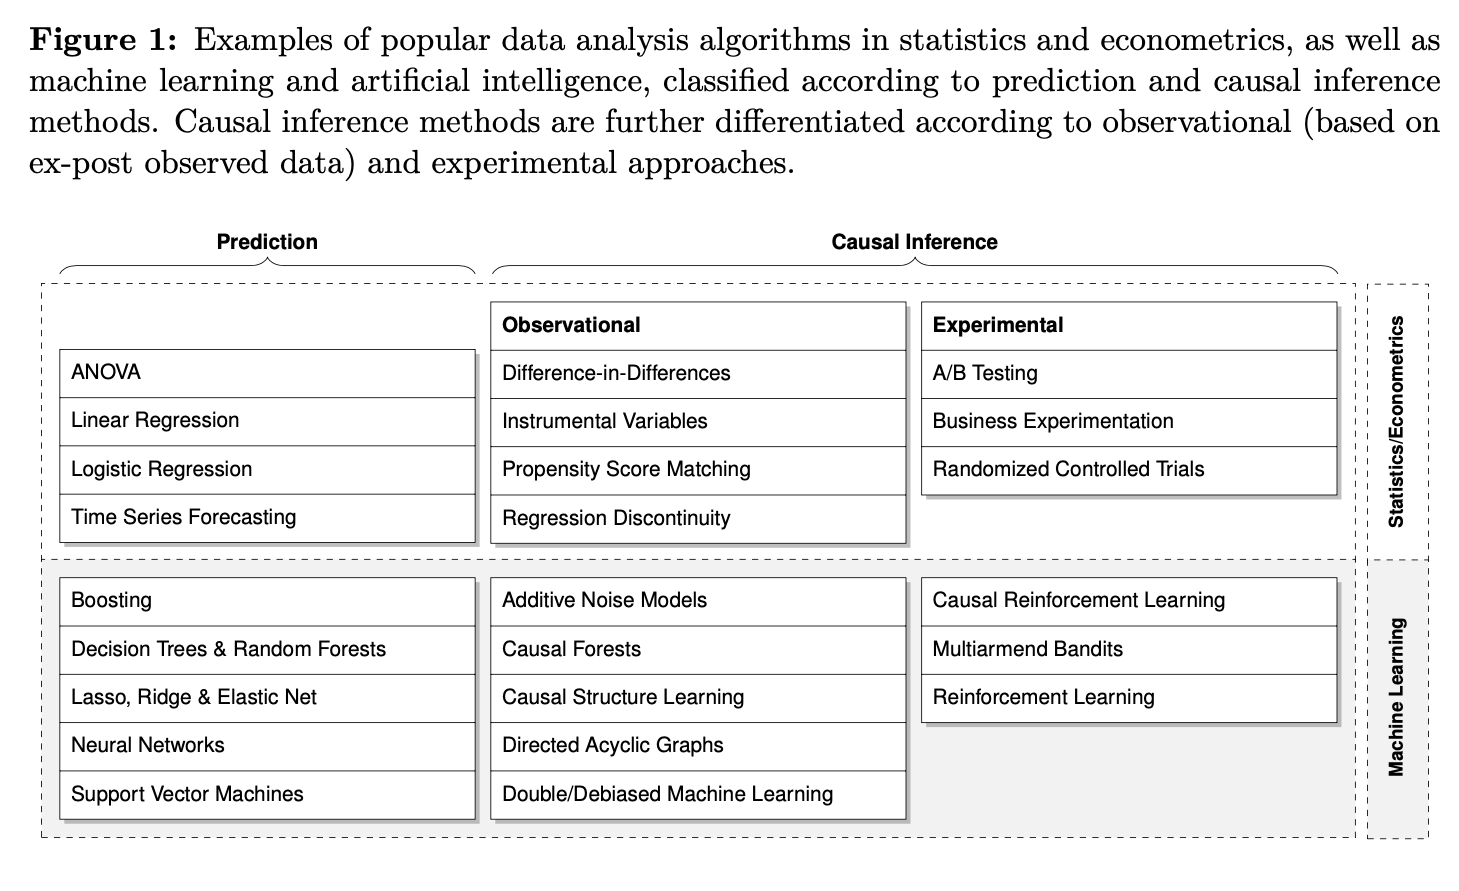
\includegraphics[scale=0.5,height=6.5cm, width=10cm]{./lecture_includes/prediction_causality.png}
\end{frame}



\begin{frame}{Potential outcomes}

\begin{itemize}
\item Conceptual framework for design based causal inference is counterfactual reasoning
\item Counterfactual modeling becomes linked to potential outcomes models with Don Rubin 1970s work on propensity scores
\item Potential outcomes notation was created by Jerzy Neyman (1923) and led Ronald Fisher (1925) to suggest RCTs
\item Huge push by Donald Rubin, a Neyman ``grandson'', in the 1970s and 1980s with Paul Rosenbaum on the propensity score
\item Guido Imbens, a Rubin coauthor, notes that it was crucial to his work on IV with Angrist, but it may even have made that work more appealing \emph{outside economics}
\url{https://youtu.be/cm8V65AS5iU?t=1097}

\end{itemize}

\end{frame}




\begin{frame}{Potential outcomes notation}

  \begin{itemize}
    \item Let the treatment be a binary variable: $$D_{i,t} =\begin{cases} 1 \text{ if hospitalized at time $t$} \\ 0 \text{ if not hospitalized at time $t$} \end{cases}$$where $i$ indexes an individual observation, such as a person
  \end{itemize}
\end{frame}

\begin{frame}{Potential outcomes notation}

  \begin{itemize}
    \item Potential outcomes: $$Y_{i,t}^j =\begin{cases} 1 \text{ health if hospitalized at time $t$} \\ 0 \text{ health if not hospitalized at time $t$} \end{cases}$$where $j$ indexes a counterfactual state of the world
  \end{itemize}
\end{frame}


\begin{frame}{Realized vs potential outcomes}

  \begin{itemize}
    \item Potential outcomes $Y^1$ are not the realized outcomes $Y$ either conceptually or notationally
    \item Potential outcomes are hypothetical states of the world but realized outcomes are \emph{ex post} the observed outcomes we have in our data due to treatment assignment
    \item This distinction is subtle, creates challenges at the introductory stage, it isn't how econometrics was historically taught, except for at the very beginning; again Imbens on this \url{https://youtu.be/cm8V65AS5iU?t=1175}
  \end{itemize}
\end{frame}



\begin{frame}{Important definitions}


  \begin{columns}[t]
    \scriptsize
    \column{.45\textwidth}

    \begin{block}{Definition 1: Individual treatment effect}
      The individual treatment effect,  $\delta_i$, equals $Y_i^1-Y_i^0$
    \end{block}
    \begin{block}{Definition 3: Fundamental problem of causal inference}
      If you need both potential outcomes to know causality with certainty, then since it is impossible to observe both $Y_i^1$ and $Y_i^0$ for the same individual, $\delta_i$, is \emph{unknowable}.
    \end{block}
    \column{.45\textwidth}
    \begin{block}{Definition 2: Switching equation}
      An individual's observed health outcomes, $Y$, is determined by treatment assignment, $D_i$, and corresponding potential outcomes:
      \begin{eqnarray*}
        Y_i& = D_iY^1_i+(1-D_i)Y^0_i& \\
        Y_i& = \begin{cases}
          Y^1_i\text{ if }D_i=1 \\
          Y^0_i\text{ if }D_i=0
        \end{cases}
      \end{eqnarray*}
    \end{block}

  \end{columns}
\end{frame}

\begin{frame}{Missing data problem}

  \begin{itemize}
    \item Causal inference is fundamentally a missing data problem requiring prediction, not of the present or the future, but of a missing past -- sometimes explicitly (nearest neighbor, synthetic control), sometimes implicitly (RDD, IV)
    \item Aggregate parameters based on individual treatment effects are descriptions of causal effects
    \item Fundamental problem of causal inference holds because of the switching equation \emph{even with big data}
  \end{itemize}

\end{frame}


\begin{frame}{Average Treatment Effects}

  \begin{block}{Definition 4: Average treatment effect (ATE)}
    The average treatment effect is the population average of all $i$ individual treatment effects
    \begin{eqnarray*}
      E[\delta_i]&=&E[Y_i^1-Y_i^0]\\
      &=&E[Y^1_i] - E[Y^0_i]
    \end{eqnarray*}
  \end{block}

  \bigskip

  Cannot be calculated because $Y^1_i$ and $Y^0_i$ do not exist \emph{for the same unit i} due to switching equation



\end{frame}



\begin{frame}{Conditional Average Treatment Effects}


  \begin{block}{Definition 5: Average Treatment Effect on the Treated (ATT)}
    The average treatment effect on the treatment group is equal to the average treatment effect conditional on being a treatment group member:
    \begin{eqnarray*}
      E[\delta|D=1]&=&E[Y^1-Y^0|D=1] \nonumber \\
      &=&E[Y^1|D=1]-E[Y^0|D=1]
    \end{eqnarray*}
  \end{block}
  Cannot be calculated because $Y^1_i$ and $Y^0_i$ do not exist \emph{for the same unit i} due to switching equation. This is the parameter we will focus on today because synthetic control \emph{only} can be used to estimate this one.


\end{frame}


\subsection{Selection bias}

\begin{frame}{Good and bad variation}

  \begin{itemize}
    \item Naive use of statistical models will often find and take advantage of all types of variation for the purpose of prediction
    \item But causal inference is much more cautious because it only uses \emph{some} of the variation
    \item This is better seen with a story and a decomposition
  \end{itemize}

\end{frame}




\begin{frame}[plain]


  \begin{block}{Definition 7: Simple difference in mean outcomes (SDO)}
    A simple difference in mean outcomes (SDO) can be approximated by the sample averages:\begin{eqnarray*}
      SDO &=& E[Y^1 | D=1] - E[Y^0 | D=0] \\
      &=& E[Y | D=1] - E[Y | D=0]
    \end{eqnarray*}
  \end{block}
  \bigskip
  I tend to use expectation operators $E[ \cdot ]$ but note we are using samples $E_N[ \cdot ]$

\end{frame}

\begin{frame}{SDO}

  \begin{itemize}
    \item Simple difference in mean outcomes is our first estimator
    \item Notice that we switched from potential outcomes to observed outcomes
    \item This means that because the SDO is based on the switching equation, it uses data
    \item So when is the SDO causal and when is it not?
  \end{itemize}

\end{frame}


\begin{frame}{Potentially biased comparisons}

  \begin{block}{Decomposition of the SDO}
    The SDO can be decomposed into the sum of three parts:
    \begin{eqnarray*}
      E[Y^1 | D=1] - E[Y^0 | D=0]&=& ATE\nonumber \\
      &&+ E[Y^0|D=1] - E[Y^0|D=0] \nonumber \\
      && + (1-\pi)(ATT - ATU)
    \end{eqnarray*}
  \end{block}
  Seeing is believing so let's work through this identity!

\end{frame}


\begin{frame}[shrink=20,plain]

  \begin{block}{Use LIE to decompose ATE into the sum of four conditional average expectations}
    \begin{eqnarray*}
      \text{ATE}&=&E[Y^1]-E[Y^0]  \\
      &=& \{\pi E[Y^1 | D=1] + (1-\pi)E[Y^1 | D=0]\}  \\
      & & - \{\pi E[Y^0|D=1] + (1-\pi) E[Y^0 | D=0]\}
    \end{eqnarray*}
  \end{block}


  \begin{block}{Substitute letters for expectations}
    \begin{eqnarray*}
      E[Y^1|D=1] &=& a  \\
      E[Y^1|D=0] &=& b  \\
      E[Y^0|D=1] &=& c  \\
      E[Y^0|D=0] &=& d  \\
      \text{ATE} &=& e
    \end{eqnarray*}
  \end{block}

  \begin{block}{Rewrite ATE}
    \begin{eqnarray*}
      e&=&\{\pi{a} + (1-\pi)b\} - \{\pi{c} + (1-\pi)d\}
    \end{eqnarray*}
  \end{block}

\end{frame}

\begin{frame}[plain]

  \begin{block}{Move SDO terms to LHS}
    \begin{eqnarray*}
      e&=&\{\pi{a} + (1-\pi)b\} - \{\pi{c} + (1-\pi)d\}  \\
      e&=&\pi{a} + b - \pi{b} - \pi{c} - d + \pi{d}  \\
      e&=&\pi{a} + b - \pi{b} - \pi{c} - d + \pi{d} + (\textbf{a} - \textbf{a}) + (\textbf{c} - \textbf{c}) + (\textbf{d} - \textbf{d})  \\
      0&=&e-\pi{a} - b + \pi{b} + \pi{c} + d - \pi{d} - \textbf{a} + \textbf{a} - \textbf{c} + \textbf{c} - \textbf{d} + \textbf{d}  \\
      \textbf{a}-\textbf{d}&=&e-\pi{a} - b + \pi{b} + \pi{c} + d - \pi{d}  + \textbf{a} - \textbf{c} + \textbf{c} - \textbf{d}  \\
      \textbf{a}-\textbf{d}&=&e  + (\textbf{c} - \textbf{d}) + \textbf{a}-\pi{a} - b + \pi{b} - \textbf{c} + \pi{c} + d - \pi{d} \\
      \textbf{a}-\textbf{d}&=&e  + (\textbf{c} - \textbf{d}) + (1-\pi)a -(1-\pi)b + (1-\pi)d - (1-\pi)c  \\
      \textbf{a}-\textbf{d}&=&e  + (\textbf{c} - \textbf{d}) + (1-\pi)(a-c) -(1-\pi)(b-d)
    \end{eqnarray*}
  \end{block}


\end{frame}

\begin{frame}[shrink=20,plain]
  \begin{block}{Rewrite from previous slide}
    \begin{eqnarray*}
      \textbf{a}-\textbf{d}&=&e  + (\textbf{c} - \textbf{d}) + (1-\pi)(a-c) -(1-\pi)(b-d)
    \end{eqnarray*}
  \end{block}

  \begin{block}{Substitute conditional means}
    \begin{eqnarray*}
      E[Y^1|D=1] - E[Y^0|D=0] &=& \text{ATE}  \\
      &&+ (E[Y^0|D=1] - E[Y^0|D=0])  \\
      && + (1-\pi)(\{E[Y^1|D=1] - \alert{E[Y^0|D=1]}\}  \\
      && - (1-\pi)\{\alert{E[Y^1|D=0]} - E[Y^0|D=0]\}) \\
      E[Y^1 | D=1] - E[Y^0 | D=0]  &=& ATE \\
      &&+ (E[Y^0|D=1] - E[Y^0|D=0])  \\
      && + (1-\pi)(ATT - ATU)
    \end{eqnarray*}
  \end{block}
\end{frame}

\begin{frame}[plain]

  \begin{block}{Decomposition of difference in means}
    \begin{eqnarray*}
      \underbrace{E_N[y_i | d_i=1] - E_N[y_i | d_i=0]}_{ \mathclap{\text{SDO}}}&=& \underbrace{E[Y^1] - E[Y^0]}_{ \mathclap{\text{Average Treatment Effect}}} \\
      &&+ \underbrace{E[Y^0|D=1] - E[Y^0 | D=0]}_{ \mathclap{\text{Selection bias}}}  \\
      && + \underbrace{(1-\pi)(ATT - ATU)}_{ \mathclap{\text{Heterogenous treatment effect bias}}}
    \end{eqnarray*}
    Using the switching equation, we get $E_N[Y|D=1] \to E[Y^1 | D=1]$, $E_N[Y|D=0] \to E[Y^0|D=0]$ and $(1-\pi)$ is the share of the population in the control group.
  \end{block}

\end{frame}

\begin{frame}{Selection bias}

  \begin{itemize}
    \item Notice this term ``selection bias'' $$E[Y^0|D=1] \neq E[Y^0 |D=0]$$
    \item Selection bias was the problem that the aliens failed to overcome -- without treatment $Y^0$, COVID patients on vents $(D=1)$ would likely have been different from those with COVID not on vents $(D=0)$
  \end{itemize}

\end{frame}




\begin{frame}{Goal of causal inference}

  Our goal in all of causal inference is to estimate aggregate causal parameters by modeling treatment assignment by \emph{imputing} missing counterfactuals

  \bigskip

This imputation process happens sometimes explicitly (nearest neighbor matching) and sometimes implicitly (RCTs)

  \bigskip

  Let's look what happens in an RCT \emph{and why} this addresses selection bias term $E[Y^0|D=1]$ and $E[Y^0|D=0]$

\end{frame}



\subsection{Independence}


\begin{frame}{Independence}


  \begin{block}{Independence assumption}
    Treatment is assigned to a population independent of that population's potential outcomes  $$(Y^0,Y^1)\independent{D}$$
  \end{block}
  This is random or quasi-random assignment and ensures mean potential outcomes for the treatment group and control group are the same.  Also ensures other variables are distributed the same for a large sample.
  \begin{eqnarray*}
    E[Y^0|D=1] &=& E[Y^0 | D=0] \\
    E[Y^1|D=1] &=& E[Y^1 | D=0]
  \end{eqnarray*}
\end{frame}

\begin{frame}{Random Assignment Solves the Selection Problem}

  \begin{eqnarray*}
    \underbrace{E_N[y_i | d_i=1] - E_N[y_i | d_i=0]}_{ \mathclap{\text{SDO}}}&=& \underbrace{E[Y^1] - E[Y^0]}_{ \mathclap{\text{Average Treatment Effect}}} \\
    &&+ \underbrace{E[Y^0|D=1] - E[Y^0 | D=0]}_{ \mathclap{\text{Selection bias}}}  \\
    && + \underbrace{(1-\pi)(ATT - ATU)}_{ \mathclap{\text{Heterogenous treatment effect bias}}}
  \end{eqnarray*}


  \begin{itemize}
    \item If treatment is independent of potential outcomes, then swap out equations and \textbf{selection bias} zeroes out:
          \begin{eqnarray*}
            E[Y^0 | D=1] - E[Y^0 | D=0] &=& 0
          \end{eqnarray*}
  \end{itemize}

\end{frame}

\begin{frame}[shrink=20,plain]
  \begin{center}
    \textbf{Random Assignment Solves the Heterogenous Treatment Effects}
  \end{center}

  \begin{itemize}
    \item How does randomization affect heterogeneity treatment effects bias from the third line?  Rewrite definitions for ATT and ATU:\begin{eqnarray*}
            \text{ATT} = E[Y^1 | D=1] - E[Y^0 | D=1] \\
            \text{ATU} = E[Y^1 | D=0] - E[Y^0 | D=0] \\
          \end{eqnarray*}
    \item Rewrite the third row bias after $1-\pi$:\begin{eqnarray*}
            ATT - ATU &=& \textbf{E[Y$^1$ $|$ D=1]} - E[Y^0 | D=1] \\
            && - \textbf{E[Y$^1$ $|$ D=0]} + E[Y^0 | D=0] \\
            &=& 0
          \end{eqnarray*}
    \item If treatment is independent of potential outcomes, then:\begin{eqnarray*}
            E_N[y_i | d_i=1] - E_N[y_i | d_i=0]  &=& E[Y^1] - E[Y^0] \\
            SDO &=& ATE
          \end{eqnarray*}
  \end{itemize}
\end{frame}




\begin{frame}{SUTVA}

  \begin{itemize}
    \item Potential outcomes model places a limit on what we can measure: the ``stable unit-treatment value assumption''
          \begin{enumerate}
            \item \textbf{S}: \emph{\textbf{s}table}
            \item \textbf{U}: across all \emph{\textbf{u}nits}, or the population
            \item \textbf{TV}: \emph{\textbf{t}reatment-value} (``treatment effect'', ``causal effect'')
            \item \textbf{A}: \emph{\textbf{a}ssumption}
          \end{enumerate}
    \item Largely about spillovers, poorly defined treatments and scale
  \end{itemize}
\end{frame}


\begin{frame}{SUTVA: No spillovers to other units}

  \begin{itemize}
    \item What if we impose a treatment at one neighborhood but not a contiguous one?
    \item Treatment may spill over causing $Y=Y^1$ even for the control units because of spillovers from treatment group
    \item Informs the design stage
  \end{itemize}
\end{frame}



\begin{frame}{SUTVA: No Hidden Variation in Treatment}

  \begin{itemize}
    \item SUTVA requires each unit receive the same treatment dosage; this is what it means by ``stable'' (i.e., notice that the super scripts contain either 0 or 1, not 0.55, 0.27)
    \item If we are estimating the effect of aspirin on headaches, we assume treatment is 200mg per person in the treatment
    \item Easy to imagine violations if hospital quality, staffing or even the vents themselves vary across treatment group
    \item Be careful what we are and are not defining as \emph{the treatment}; you may have to think of it as multiple arms
  \end{itemize}
\end{frame}

\begin{frame}{SUTVA: Scale can affect stability of treatment effects}

  Easier to imagine this with a different example.
  \begin{itemize}
    \item Let's say we estimate a causal effect of early childhood intervention in Texas
    \item Now President Biden wants to roll it out for the whole United States -- will it have the same effect as we found?
    \item Scaling up a policy can be challenging to predict if there are rising costs of production
    \item What if expansion requires hiring lower quality teachers just to make classes?
    \item That's a general equilibrium effect; we only estimated a partial equilibrium effect (external versus internal validity)
  \end{itemize}
\end{frame}
% \input{lectures_fisher.tex}


\subsection{Example of physical experimentation: eBay advertising}

\begin{frame}

\begin{figure}[hpt]
\begin{center}
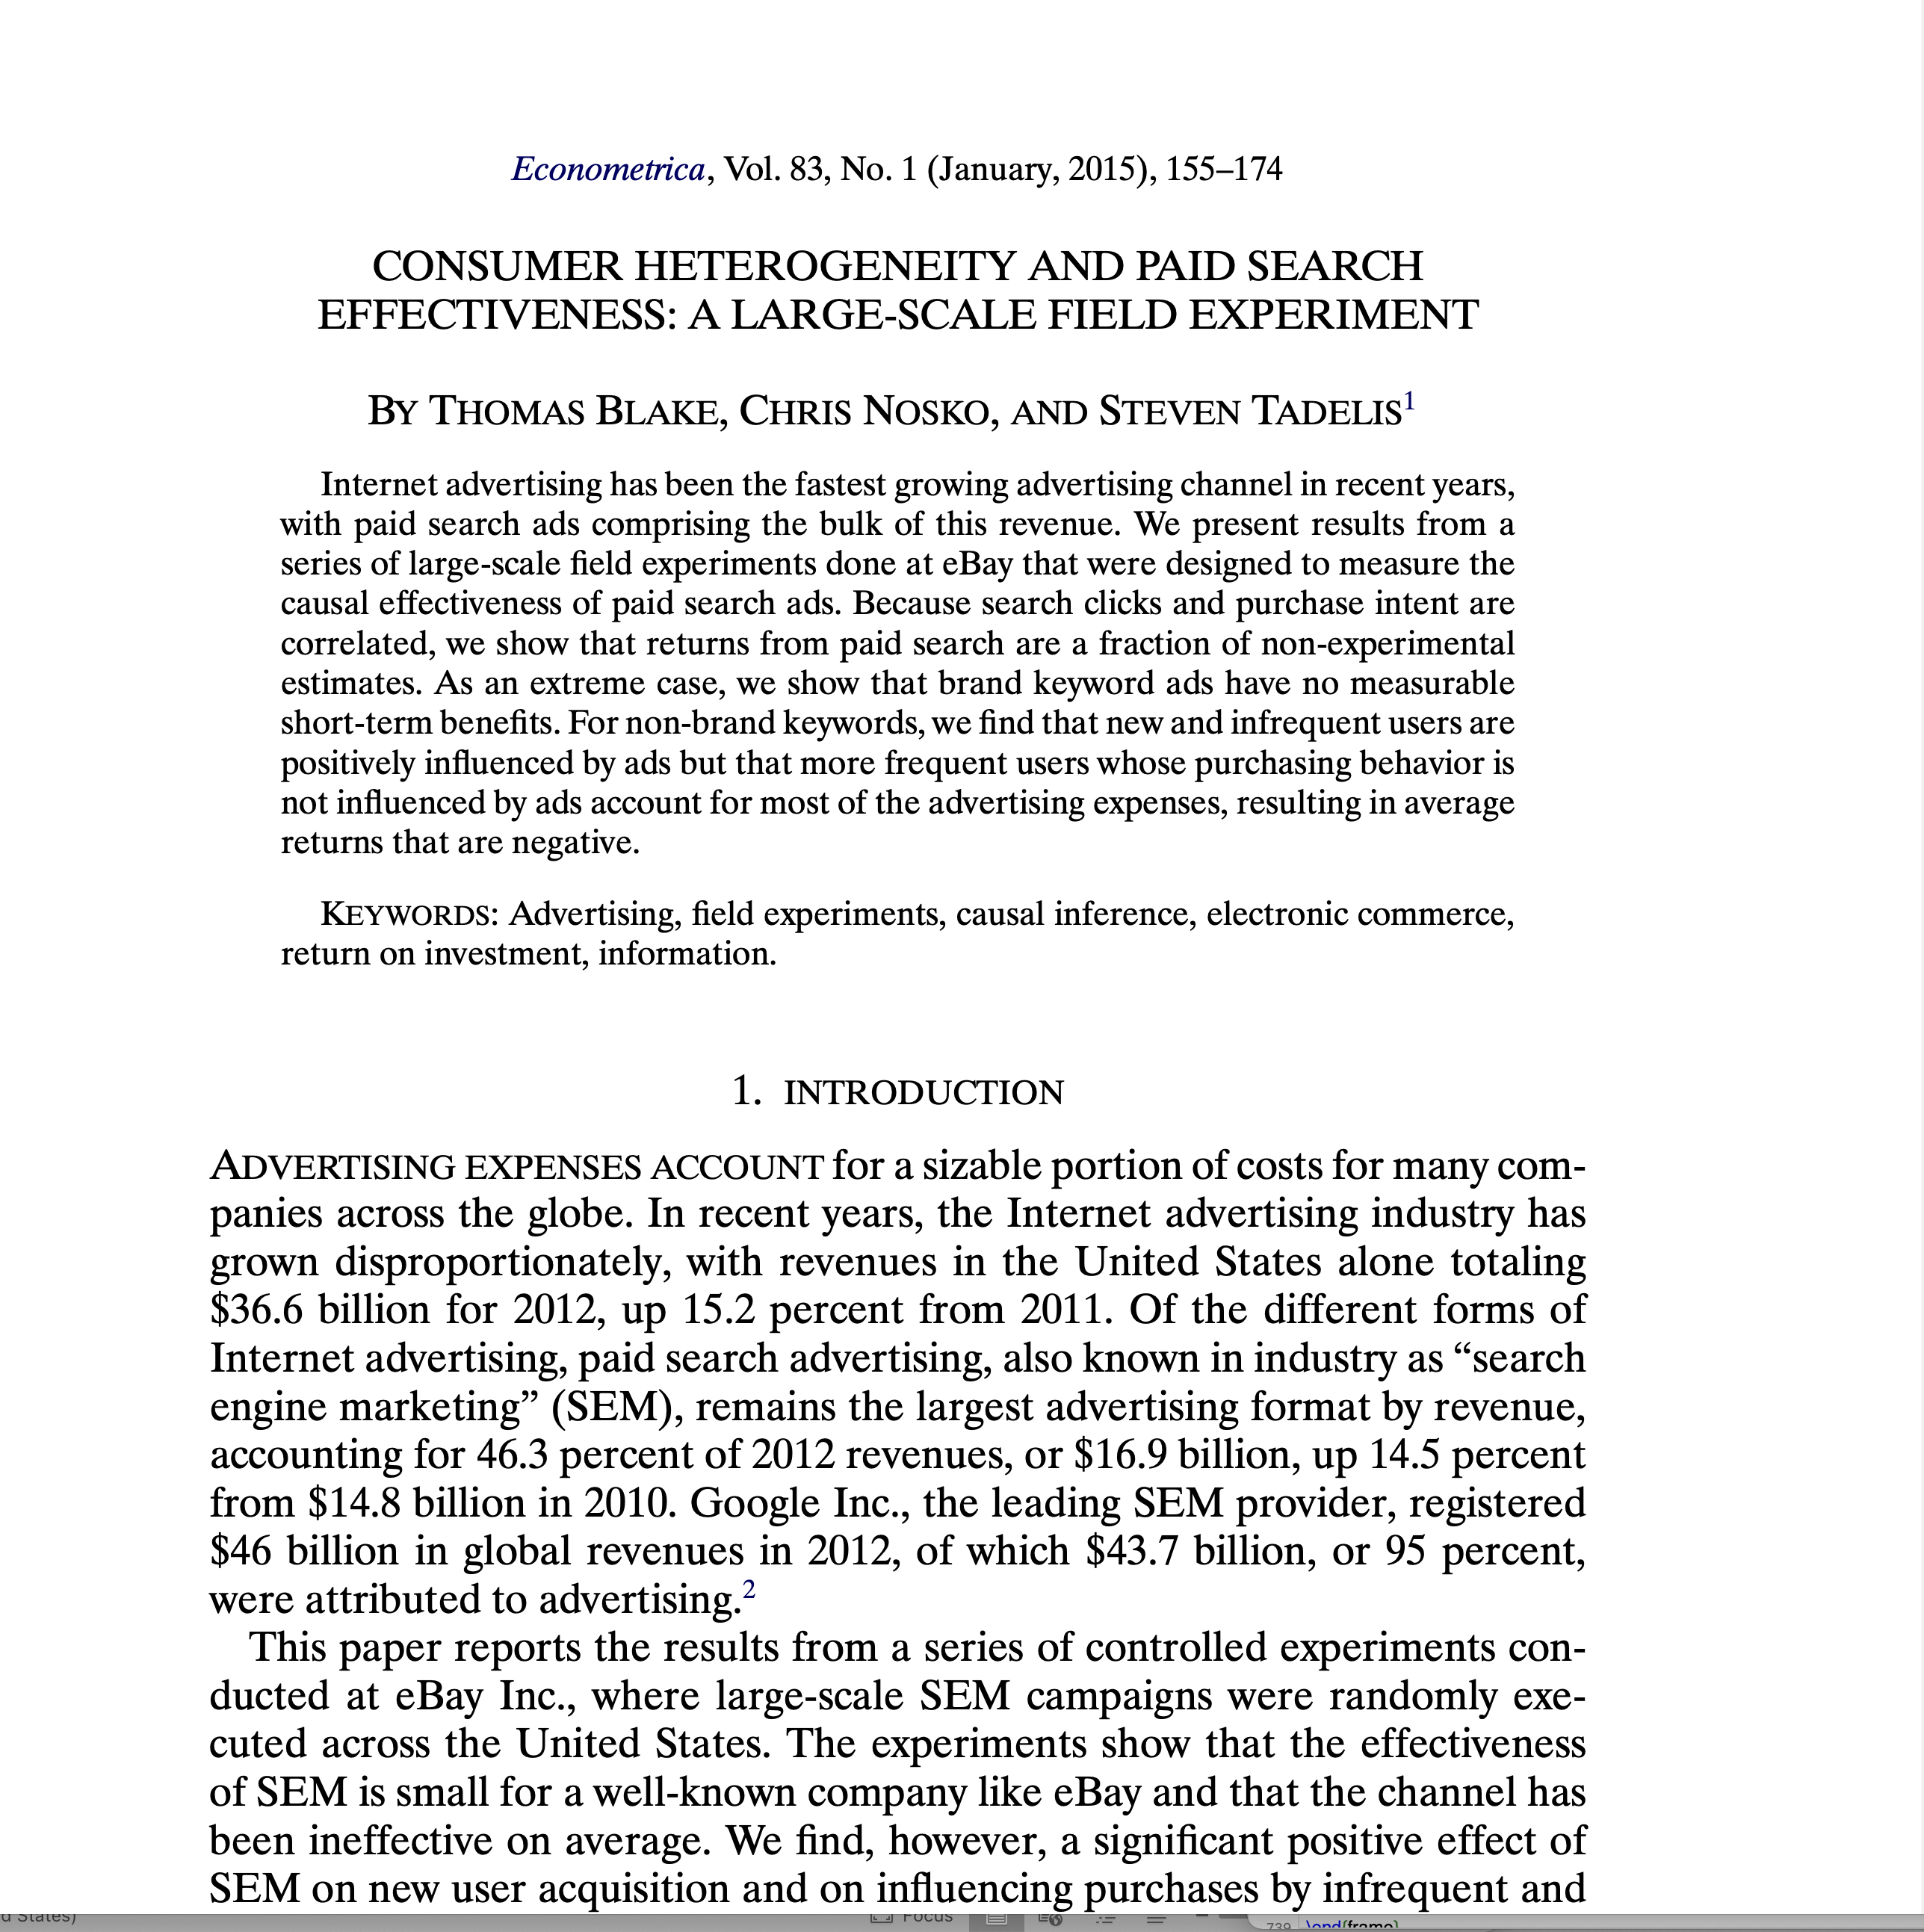
\includegraphics[scale=0.25]{./lecture_includes/econometrica_steve.png}
\end{center}
\end{figure}

\end{frame}

\begin{frame}{Internet advertising facts}

\begin{itemize}
\item In 2012, revenues from Internet advertising was \$36.6 billion and has only grown since
\item Paid search (``search engine marketing'') is the largest format by revenue (46.3\% of 2012 revenues, or \$16.9 billion)
\item Google is leading provider (registered \$46 billion in global revenues in 2012 of which 95\% was attributed to advertising)
\end{itemize}

\end{frame}

\begin{frame}{Selection bias}

\begin{itemize}
\item Treatment was targeted ads at particular people conducting particular types of keyword search
\item Consumers who choose to click on ads are loyal and already informed about products with high likelihood to buy already 
\item Problem is ads are targeting people at the end of their search, so the question is whether they would've found it already (i.e., $E[Y^0|D=1] \neq E[Y^0|D=0]$)
\end{itemize}


\end{frame}



\begin{frame}{Selection bias}

\begin{itemize}
\item Estimated return on investment using OLS  found ROI of over 1600\%
\item Compared this to experimental methods and found ROI of -63\% with a 95\% CI of $[-124\%, -3\%]$, rejecting the hypothesis that the channel yielded short-run positive returns
\item Think back to perfect doctor -- Even without the treatment ($Y^0$), the treated group observationally would've still found a way
\end{itemize}

\end{frame}

\begin{frame}{Natural experiment}

\begin{itemize}
\item Study began with a naturally occurring and somewhat fortuitous  event at eBay
\item eBay halted SEM queries for brand words (i.e., queries that included the term eBay) on Yahoo! and Microsoft but continued to pay for these terms on Google
\item Blake, Nosky and Tadelis (2015) showed almost all of the foregone click traffic and attributed sales were captured by natural search
\item Substitution between paid and unpaid traffic was nearly one to one complete
\end{itemize}

\end{frame}


\begin{frame}

\begin{figure}
\begin{center}
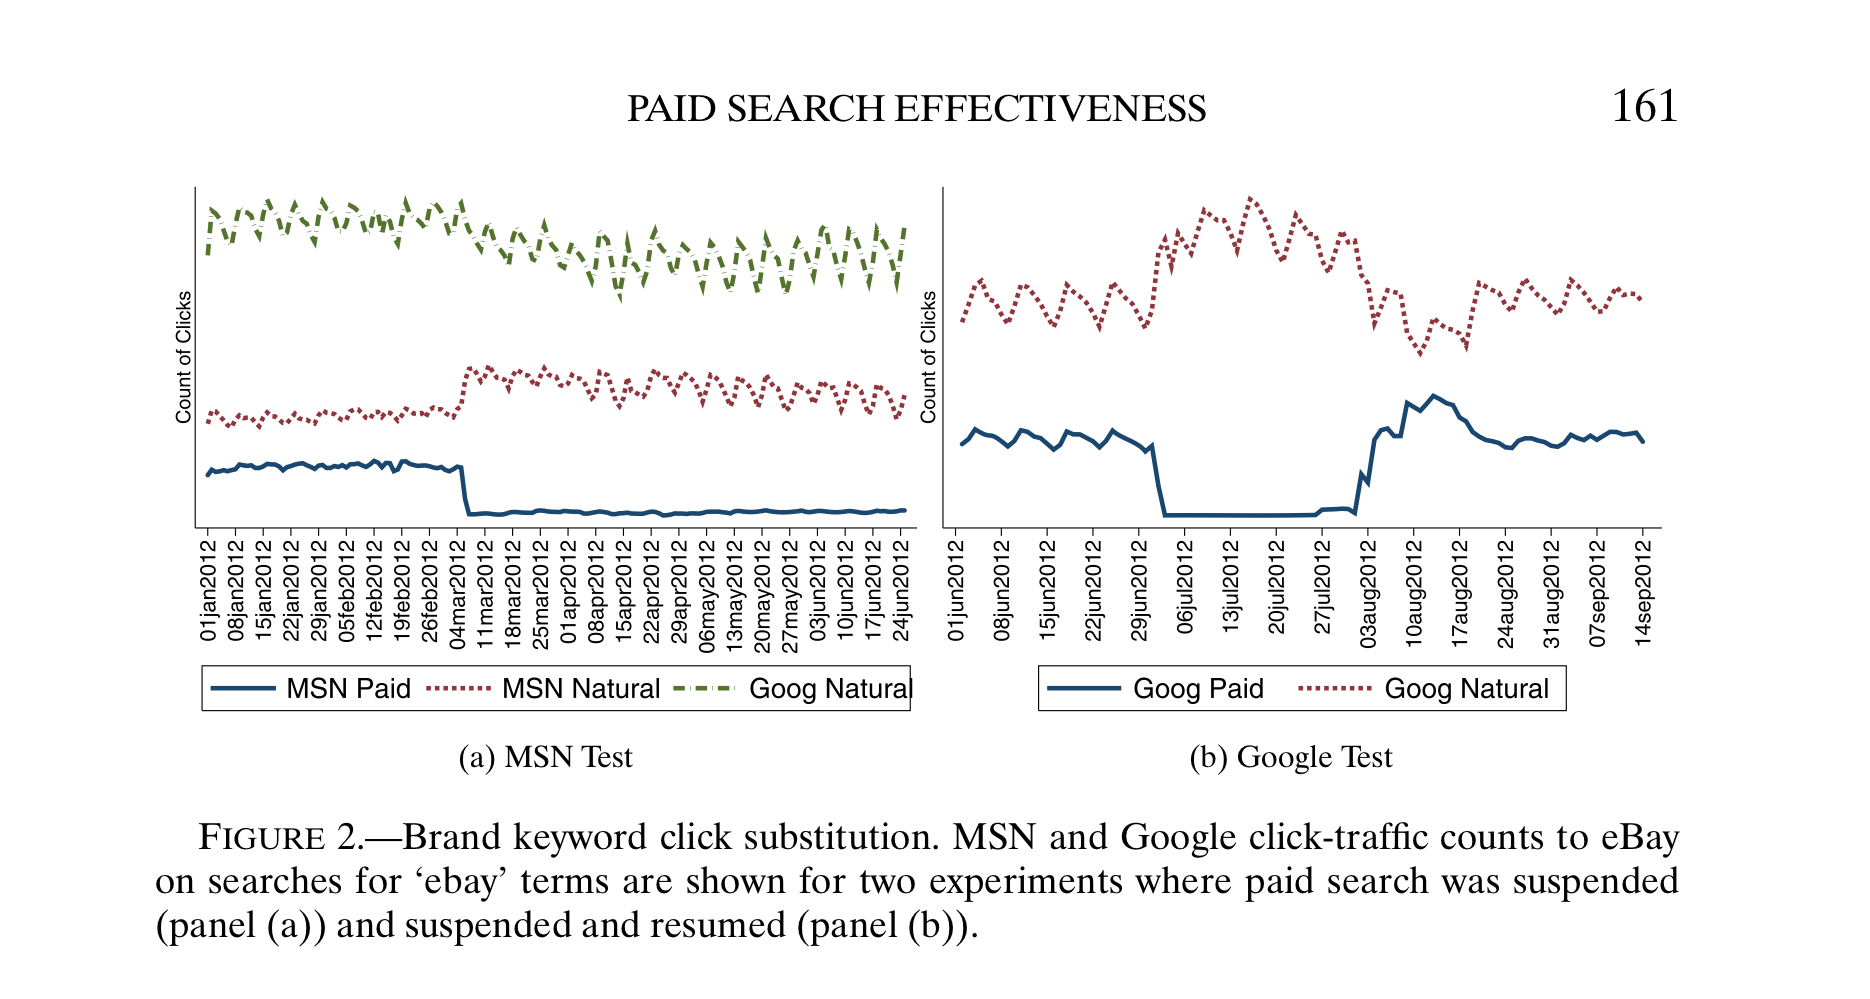
\includegraphics[scale=0.2]{./lecture_includes/tadelis_fig1.png}
\end{center}
\end{figure}

\end{frame}

\begin{frame}{Interpretation of natural experiment}

\begin{quote}
``The evidence strongly supports the intuitive notion that for brand keywords, natural search is close to a perfect substitute for paid search, making brand keyword SEM ineffective for short-term sales.  After all, the users who type the brand keyword in the search query intend to reach the company's website, and most likely will execute on their intent regardless of the appearance of a paid search ad.''
\end{quote}

\end{frame}

\begin{frame}{Selection bias}

Observational data masked causal effect (recall the decomposition of the any non-designed estimation strategy)

\bigskip

\begin{quote}
``Advertising may appear to attract these consumers, when in reality they would have found other channels to visit the company's website.  We overcome this endogeneity challenge with our controlled experiments.''
\end{quote}

\end{frame}




\begin{frame}{RCT}

Natural experiment was valuable, but eBay could run a large scale RCT.

\bigskip


Use this finding of a nearly one-to-one substitution once paid search was dropped to convince eBay to field a large scale RCT discontinuing non-band key words

\bigskip


\end{frame}

\begin{frame}{Design of the experiment}

\begin{itemize}
\item Randomly assigned 30 percent of eBay's US traffic to stop all bidding for all non-brand keywords for 60 days
\item Some random group of users, in other words, were exposed to ads; a control group did not see the ads
\item Used Google's geographic bid feature that can accurately identify geographic market of the user conducting the search
\item Ads were suspended in 30 percent of markets to reduce the scope of the test and minimize the potential cost and impact to the business
\end{itemize}

\end{frame}

\begin{frame}

\begin{figure}
\begin{center}
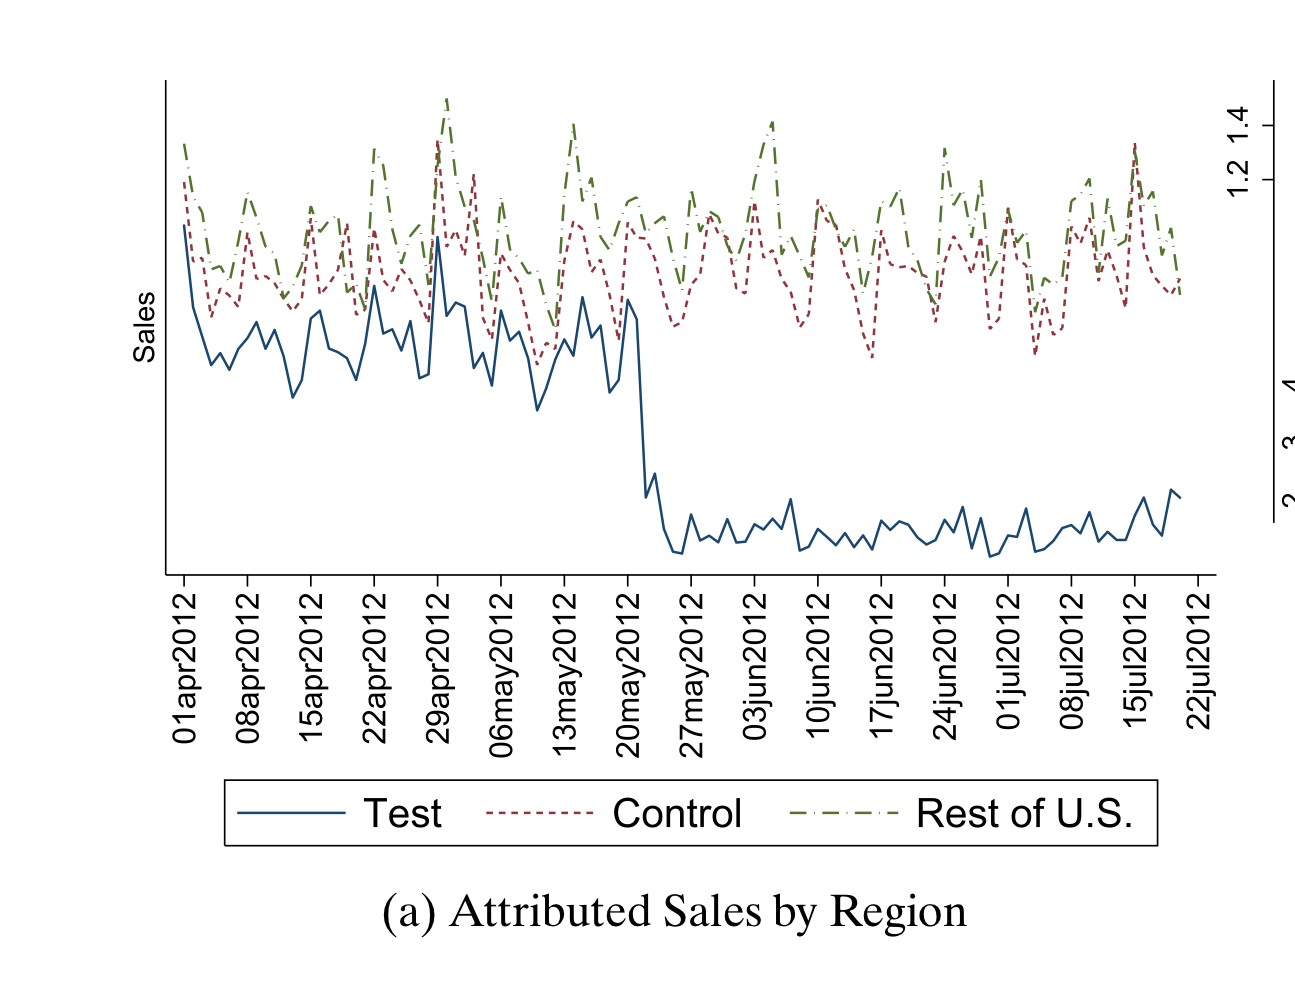
\includegraphics[scale=0.2]{./lecture_includes/tadelis_fig3.png}
\caption{Attributed sales due to clicking on a Google link (treatment group)}
\end{center}
\end{figure}

\end{frame}


\begin{frame}

\begin{figure}
\begin{center}
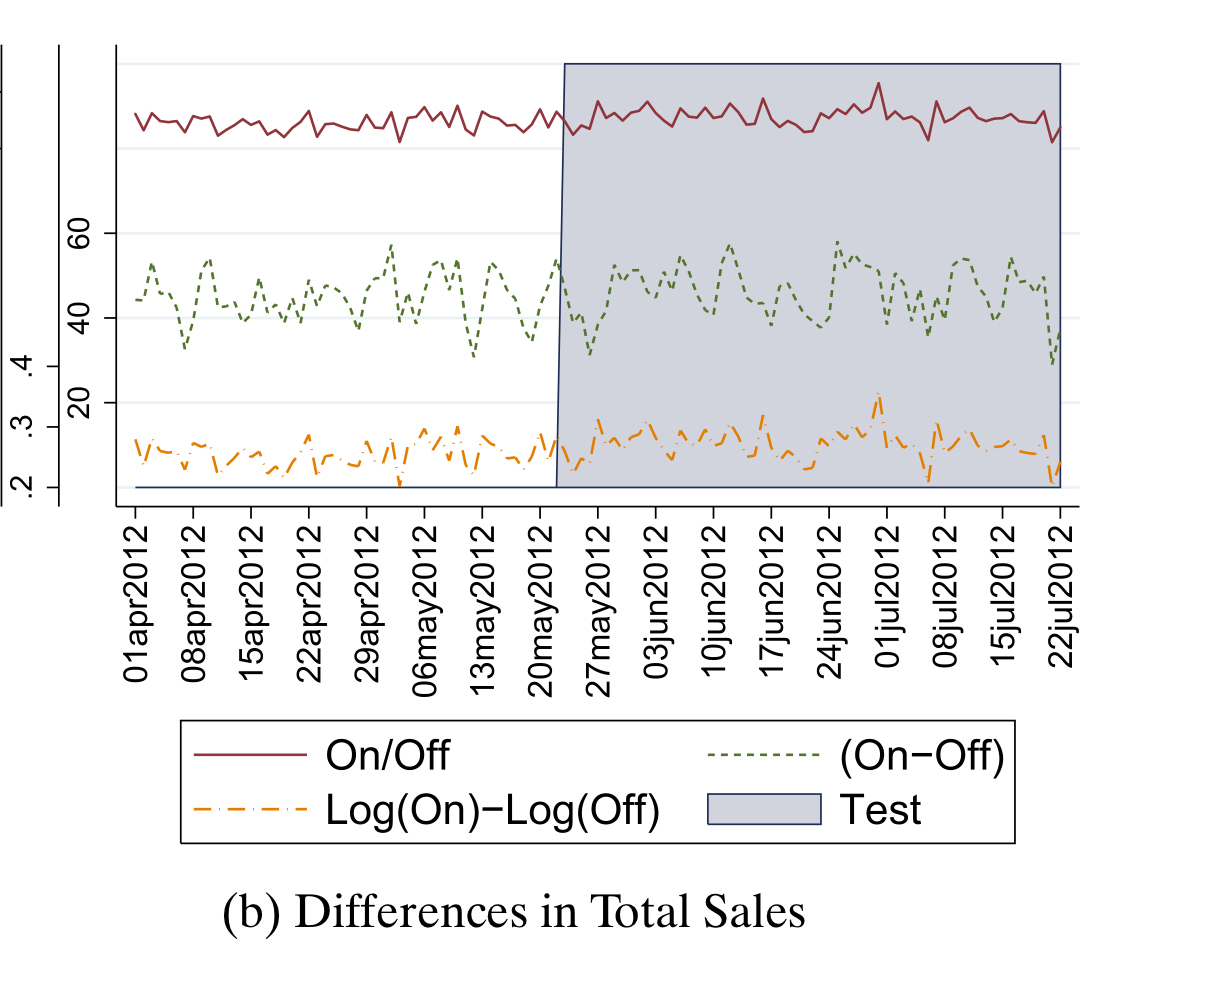
\includegraphics[scale=0.2]{./lecture_includes/tadelis_fig2.png}
\caption{Differences in total sales by market (treatment to control)}
\end{center}
\end{figure}

\end{frame}

\begin{frame}

\begin{figure}
\begin{center}
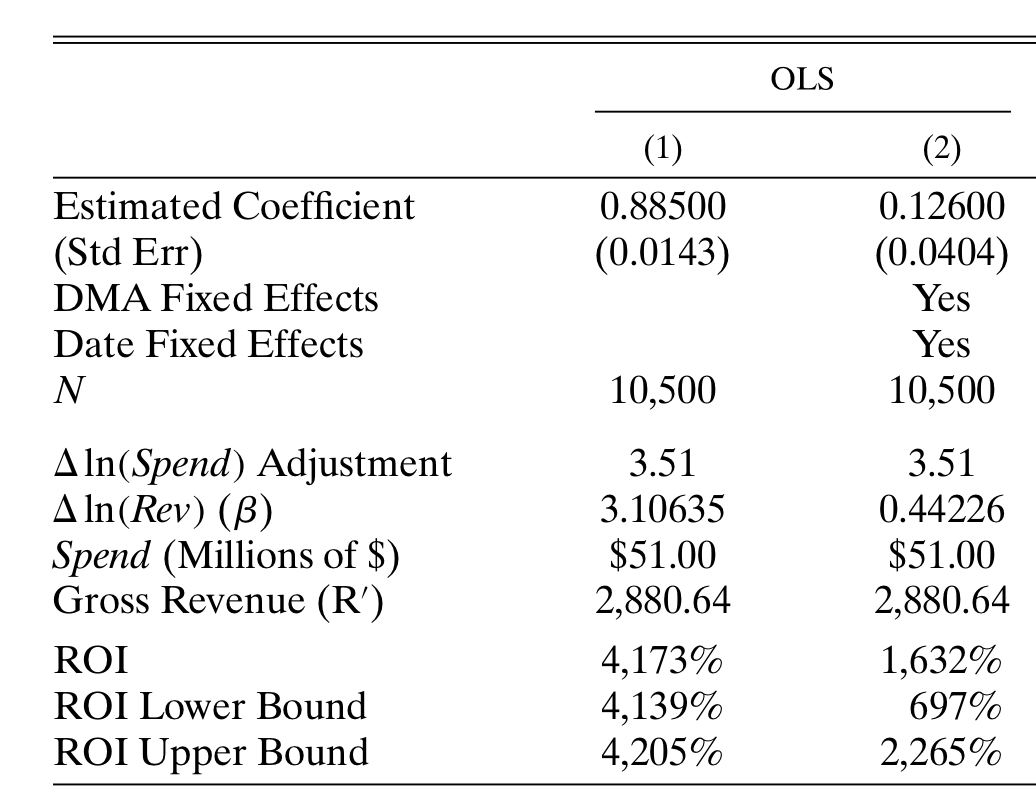
\includegraphics[scale=0.2]{./lecture_includes/tadelis_ols1.png}
\caption{Spending effect on revenue using OLS but not the randomization. Effects are gigantic. }
\end{center}
\end{figure}

\end{frame}

\begin{frame}

\begin{figure}
\begin{center}
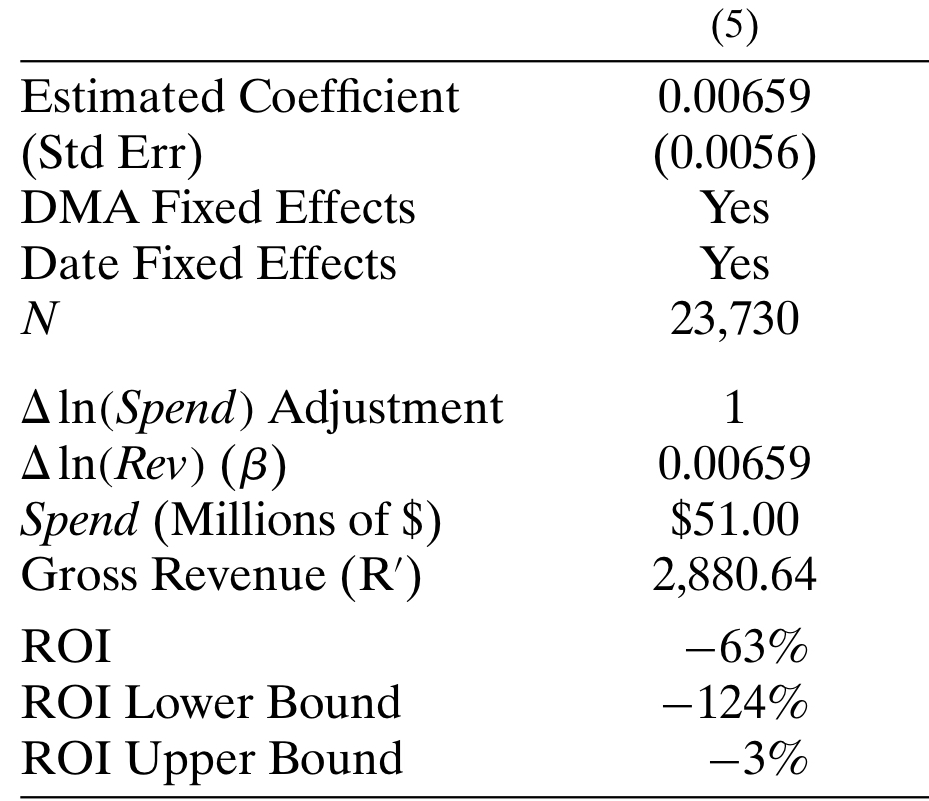
\includegraphics[scale=0.2]{./lecture_includes/tadelis_ols2.png}
\caption{Spending effect on revenue using the randomization. Effects are negative. }
\end{center}
\end{figure}

\end{frame}

\begin{frame}{Heterogenous treatment effects}

\begin{itemize}
\item Recall how the potential outcomes model explicitly models individual treatment effects could be unique and that the perfect doctor showed selection on gains masked treatment effects, perhaps even reversing sign
\item Search advertising in this RCT only worked if the consumer had no idea that the company had the desired product
\item Large firms like eBay with powerful brands will see little benefit from paid search advertising because most consumers already know that they exist, as well as what they have to offer
\end{itemize}

\end{frame}


\begin{frame}

\begin{figure}
\begin{center}
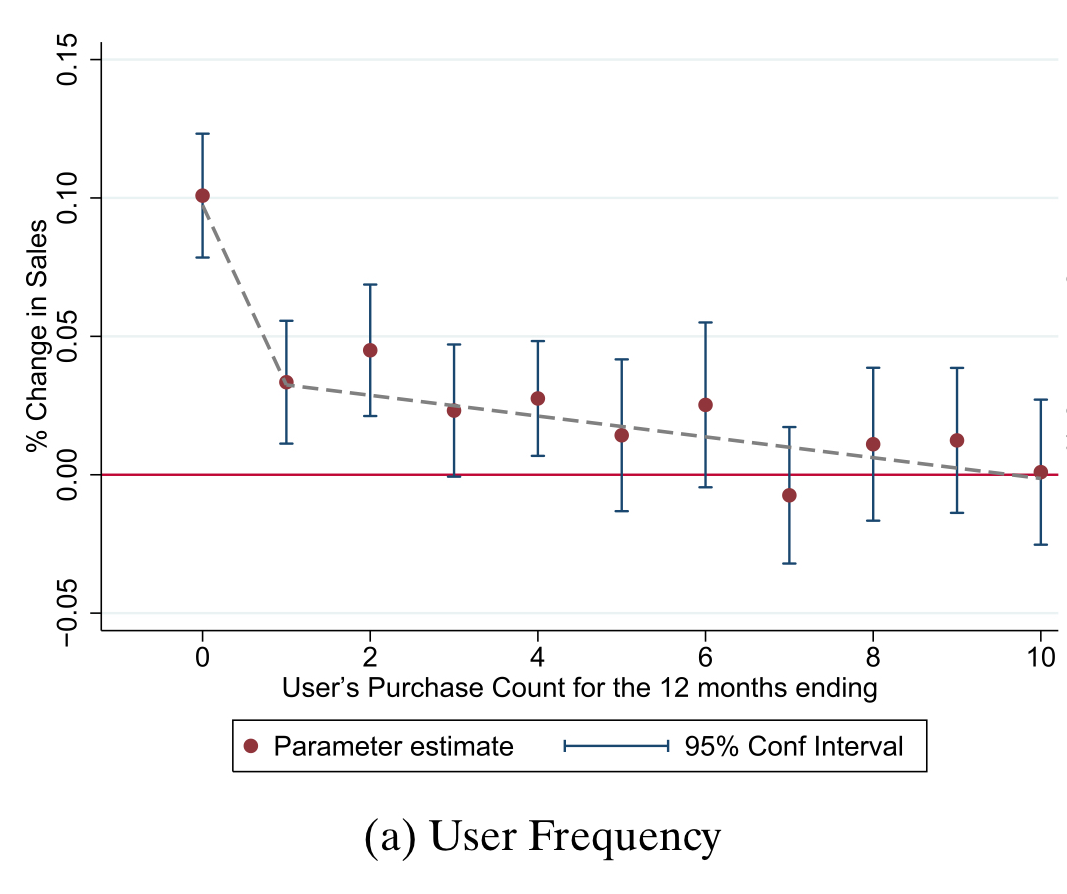
\includegraphics[scale=0.2]{./lecture_includes/tadelis_newuser_fig1.png}
\caption{Effects on new users are positive and large, but not others. }
\end{center}
\end{figure}

\end{frame}

\begin{frame}

\begin{figure}
\begin{center}
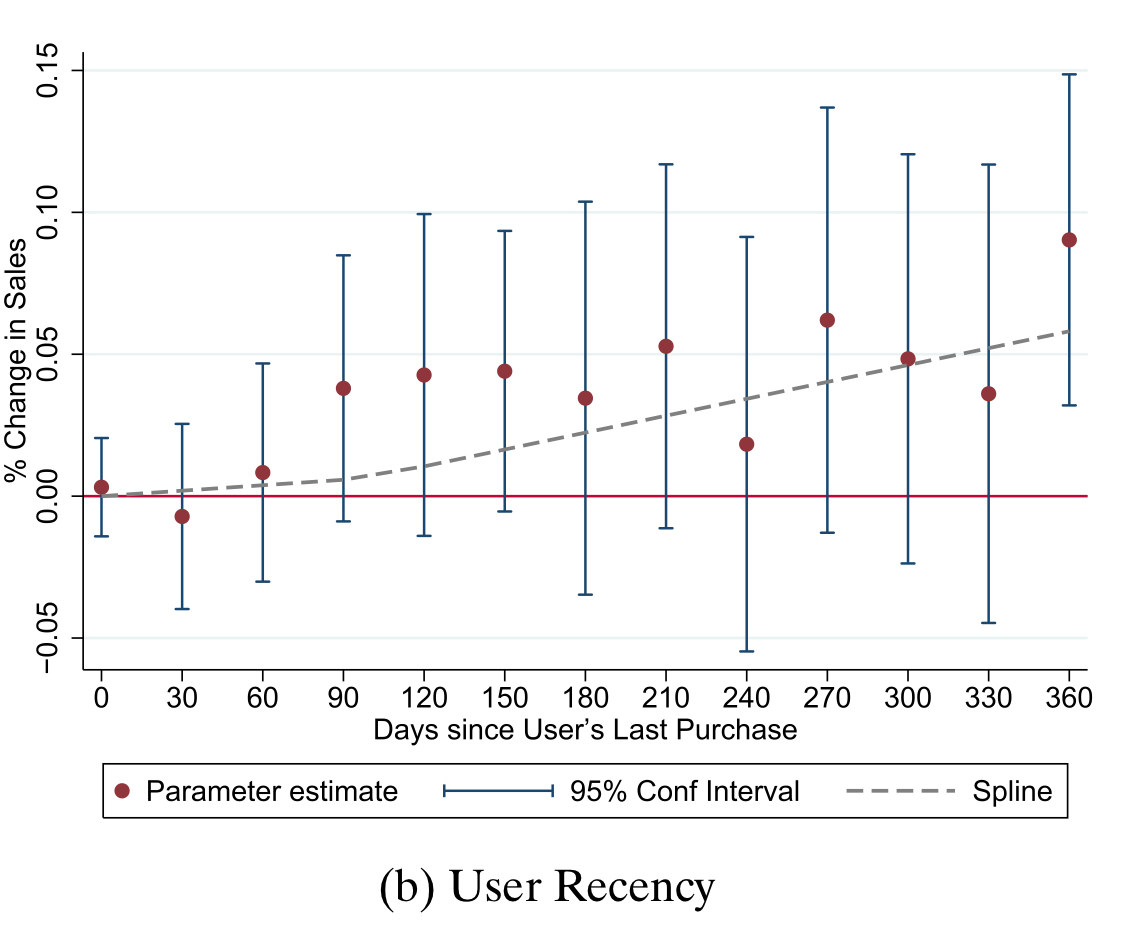
\includegraphics[scale=0.2]{./lecture_includes/tadelis_newuser_fig2.png}
\caption{Effects are largest for ``least active'' customers. }
\end{center}
\end{figure}

\end{frame}


\begin{frame}{Why are causal effects small?}

\begin{itemize}
\item They suggest that the brand query tests found small causal returns because users simply substituted from the paid search clicks to the natural search clicks
\item If that's the case, then it's explicitly a selection bias story $$E[Y^0|D=1] \neq E[Y^0|D=0]$$ where $D$ is being shown the branded advertisement based on search (i.e., they were already going there)
\item They weren't using branded search for information; they were using to \emph{navigate}
\end{itemize}

\end{frame}

\begin{frame}{Self selection based on gains}

\begin{itemize}
\item OLS was biased, not because OLS was bad because the comparisons were bad (under randomization, OLS is fine)
\item Potential outcomes is the foundation of the physical experiment because the physical experiment assigns units to treatments \emph{independent} of potential outcomes, $Y^0,Y^1$
\item This is important because outside of the physical experiment, we expect people select those important treatments based on whether, subjectively, they think $Y^1>Y^0$ or $Y^1\leq Y^0$. 
\item Rational actors almost by definition are thought to ``self-select into treatment'' making non-designed comparisons potentially misleading -- sometimes by a little, sometimes by a lot
\end{itemize}

\end{frame}


\begin{frame}{Next: Synthetic control}

\begin{itemize}

\item Very hard to imagine a situation where randomization wouldn't help us solve this identification problem, if not completely solve it altogether
\item But unfortunately, many problems we simply cannot overcome with randomization -- not because it's scientifically undesirable, but \emph{because no one will let us randomize!}
\item Next we will look at a particular method that attempts to address the problem of causal inference by finding a set of peers that approximate the counterfactual -- the synthetic control
\end{itemize}

\end{frame}




\end{document}
\begin{frame}{Angrist and Imbens and the 1990s}

  \begin{itemize}
    \item Angrist writes a dissertation using randomized instruments (Vietnam draft), goes to Harvard, overlaps with Imbens for a year, they are mentored by Gary Chamberlain, work with Don Rubin, write their famous LATE paper
    \item Chamberlain recommends potential outcomes framework over a different one that had been used at that time (latent index) and that seems to make the work more generally attractive (like to Rubin)
    \item Let's spend twenty minutes listening to them
  \end{itemize}

\end{frame}

\begin{frame}{Angrist, Imbens and Harvard}


  Josh Angrist on the negative results at the time (10 min)

  \url{https://youtu.be/ApNtXe-JDfA?t=1885}


  \bigskip
  Guido Imbens on the reception of their work (10 min)

  \url{https://youtu.be/cm8V65AS5iU?t=799}

\end{frame}
